\chapter{Introduction}

Rise is a tabletop role-playing game.
This chapter explains what that means, and how Rise is different from other existing games.

\section{What Is A Tabletop Role-Playing Game?}
  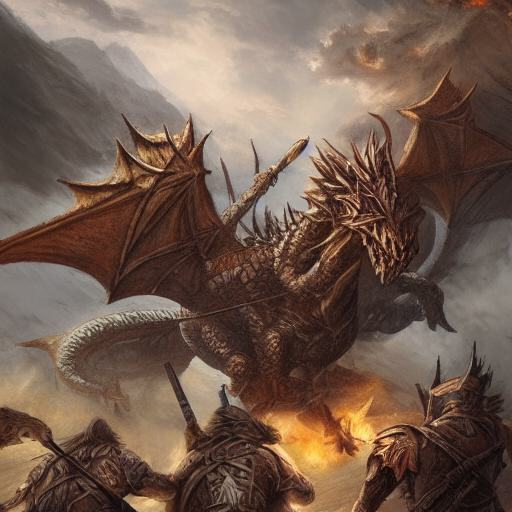
\includegraphics[width=\columnwidth]{introduction/what is a tabletop rpg}
  In tabletop role-playing games like Rise, you play a specific character of your own design.
  Your character can try to do anything you can imagine in a world that the game master, or GM, creates.
  Of course, you won't always succeed.
  The details of your character's capabilities are defined in the pages ahead; when you're done creating a character, it will have a personality of its own, along with strengths, weaknesses, and special abilities.
  Usually, your character will go on adventures with other characters, each of which is played by other players.
  Together, you will create and experience a story with the Game Master, or GM, who defines the universe that the player characters inhabit.

  \subsection{Describing Actions}
    Most of the time, when you're playing a game of Rise, you simply describe what you want your character to do.
    For example, you can say that your character steps out of their room in the inn and walks over to knock on a friend's door.
    Although Rise has rules that could govern some aspects of that scenario, such as an Awareness check to see if your friend notices you knocking, you wouldn't usually reference those rules explicitly.
    Even in the unlikely scenario that your friend doesn't notice you knock the first time, you can just knock again, so there's no point in worrying about the details.
    If something seems reasonable, it probably is, and you don't need to worry about the fiddly bits.

    Sometimes, when you describe what your character tries to do, the action has a narratively relevant chance of failure.
    Instead of knocking on the door to say hi, you might only have time to bang on it once to warn your sleeping friend about an attack from assassins.
    In that case, there's some chance that your friend is sleeping too deeply to notice the noise the first time you knock.
    You could try knocking again, just like in the first scenario, but in this scenario that failure would cost you valuable time to survive the attack.
    In that scenario, you would roll a die to determine whether you succeed in your action - or in this case, whether your friend would succeed in their attempt to notice you.

  \subsection{Using Specific Abilities}
    Instead of describing broadly what you want to have happen, you might choose one of a list of clearly defined abilities that your character can use.
    Every character has specific abilities unique to them, such as a wizard's spells known.
    There are also a number of simple abilities that anyone can use, such as the \ability{dirty trick} or \ability{trip} abilities.
    These universal abilities attempt to adequately describe a wide variety of reasonable improvised actions that you might try to use in combat.

    Explicitly defined abilities have rules for determining what happens when you use them.
    Some abilities, such as attacks in combat, require rolling dice to determine how effective they are.
    Of course, you can use your character's abilities at any time, not just in combat.
    Abilities such as the \spell{create water} or \spell{distant hand} spells can be used to solve other kinds of problems entirely.

  \subsection{Rolling Dice}
    Eventually, you'll have to determine whether something succeeds or fails.
    This can happen as part of using a specific ability that tells you exactly what to roll, or because you tried to narrate your character taking an action that has a dramatically relevant chance of failure.
    In either case, you'll roll a single ten-sided die, also known as 1d10.
    You'll add some modifier that represents how skilled your character is at the particular thing that they are trying to do.
    At the GM's discretion, they may also give the roll an extra bonus or penalty based on the circumstances that your character is in.
    If your die roll is high enough, your character succeeds at whatever they were trying to do.
    Otherwise, your character fails, which may sometimes have additional consequences.

    In Rise, it's entirely possible for characters to be so skilled that they succeed at what they are trying to do even if you roll a 1.
    Likewise, there are tasks that are so obviously impossible for your character that they cannot possibly succeed.
    In those cases, there's no reason to roll!
    Of course, the GM is the final arbiter of whether rolling is necessary.
    They may have information that the players do not.

    In some cases, you roll multiple dice at once.
    A collection of dice is called a \glossterm{dice pool}.
    Dice pools are written with the number of dice, followed by ``d'', followed by the size of dice to roll.
    For example, 2d6 means you roll two six-sided dice.

  \subsection{Why Use So Many Rules?}
    
\includegraphics[width=\columnwidth]{introduction/so many rules}

    Tabletop role-playing games attempt to create rules to define how their universe works.
    Some games are intentionally vague or minimalist about their rules, which can be fun!
    Simple games are easy to start playing, and they try to avoid getting in the way of good role-playing.
    However, Rise takes a different approach.
    It spends a lot of effort - and words - attempting to define an internally consistent universe, and creating a large number of specific abilities that can be used in that universe.
    There are a few important advantages to taking this approach: establishing expectations, supporting multiple play styles, and assisting the GM.

    \subsubsection{Establishing Expectations}
      Different people can have very different ideas about what is realistic - or narratively appropriate - in a made-up fantasy universe.
      To some people, kicking in the tavern door and starting a brawl is just some good clean fun, and you'll take a few good punches and then laugh about it later that evening over drinks.
      But to other people, that might sound like a good way to find yourself imprisoned for the foreseeable future with all of your possessions confiscated by the town guard.
      Another interpretation of that scenario might see the brawler seriously injured with a broken bottle in the eye, leaving them partially blinded for weeks - or indefinitely.

      All of those ideas are valid, and they each match the narrative of a particular type of story.
      However, it's important that everyone sitting at a table and playing a game agrees about what to expect.
      Players can get confused or frustrated when their actions have consequences that feel arbitrary or unfair.
      Generally, games are more fun if everyone in the game shares a common set of expectations and conventions.
      Otherwise, games can devolve into disagreements about what is or isn't reasonable.

      One way to establish these expectations is to use a rules system like Rise that defines some expectations explicitly.
      If the scenario above happened in Rise, the last outcome of an incapacitating bottle to the eye shouldn't normally be possible, since the rules explicitly define how injury works.
      Knowing what is and isn't possible can help give players and GMs a useful set of guardrails for what they try to do in the universe.
      It's relatively easy to get everyone to agree about simple things that regular human people have experience with, like how difficult it is to climb a tree.
      However, Rise is full of superhuman people and monsters, and eventually you'll need to figure out how far a barbarian as strong as Hercules can throw a bear.
      Having a single authoritative resource to consult can cut off long disagreements about details that are difficult or impossible to determine objectively.

      Of course, different games played with a flexible rules system like Rise can have very different tones and themes.
      Either of the first two scenarios in the tavern are still plausible in different games, and a GM can use house rules to make vital wounds have more long-term consequences if they want.
      Using a rules system like Rise can help, but it is not the full answer by itself.
      The GM and players always share responsibility for establishing expectations about what genre a game will be, and conforming to those expectations to the extent that it makes the game more fun.

    \subsubsection{Supporting Multiple Play Styles}
      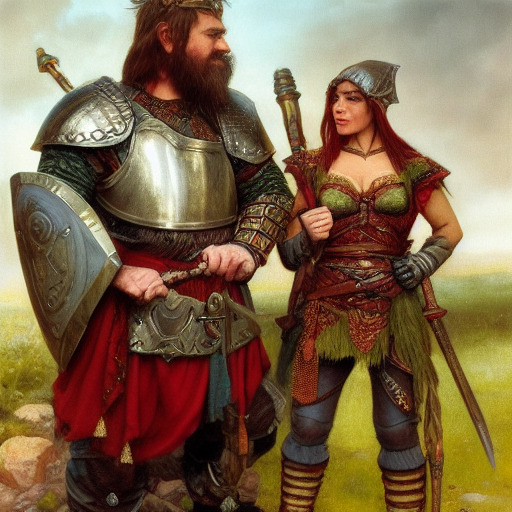
\includegraphics[width=\columnwidth]{introduction/multiple play styles}
      Some people deeply enjoy the process of role-playing itself.
      They enjoy the process of getting into a character and speaking in their voice, exploring their needs and desires, and building a narrative for them over time.
      These people often do not need the confines of a robust rules system, and can play equally well in games with minimal rules or none at all.

      Other people do not enjoy role-playing as an end in itself, or even at all.
      However, they may still enjoy the \textit{game} aspect of a role-playing game.
      Instead of playing a character for their personality and backstory, they may play a character for their unique mechanics and tactical advantages.

      Still other people may be interested in role-playing as a concept, but find it daunting.
      The blank page in front of you when you start painting a picture or writing an essay can be daunting, and that first step is often the hardest to take.
      Giving people a clearly defined set of abilities and specific tools for interacting with the world can enhance creativity by providing a safe space for interaction and experimentation.
      Even if you don't enjoy or feel confident in speaking in your character's voice, you can still engage with the narrative aspects of the adventure by casting a relevant spell or making a relevant skill check.
      People in this middle ground can sometimes enjoy deeper role-playing games while being feeling lost in role-playing games with minimal or nonexistent rules.

      One of the joys - and challenges - of Rise is drawing together people with very different desires and play styles to share a single experience.
      Rules-free role-playing games and tactical wargames can both have a narrower appeal than rules-heavy role-playing games like Rise, which try to provide something for everyone.
      You can run games with deep role-players alongside tactical gamers, and it can be a lot of fun.
      It does place a greater burden on the GM to provide the right ratio of content to keep everyone happy, and it does require the players to be patient when their preferred playstyle is put in the background to support the needs of other players.
      A well-blended game can also draw people out of their comfort zones slowly and safely over time as they observe and start to enjoy the playstyles of the other players in the game.

    \subsubsection{Assisting the GM}
      The Game Master carries an extra weight of responsibility to shape the flow of the game.
      Creating narratively consistent universes, appropriate challenges, and engaging storylines out of thin air is deeply challenging.
      If this job is too difficult, no one will want to do it, and then no one will play the game!
      Making the GM's job easier is a critical component of any role-playing game.

      There are several ways that Rise can make the GM's job easier.
      It provides information about the mechanics and tropes of the universe that the game takes place in, which helps establish expectations and resolve disputes that might come up during the game.
      It will provide a clear narrative foundation for the world and the characters in that world, which minimizes the up-front work required to run a game, once that section of the book is more complete.
      It will provide a wealth of pre-packaged challenges appropriate for players of any power level or play style, and advice for how to use those challenges appropriately, once that section of the book is more complete.
      The GM-focused sections are currently the most unfinished part of Rise, and this will be a more useful guide before Rise is done.

\section{What Makes Rise Different?}
  If you haven't played other tabletop role-playing games, feel free to skip this section.
  If you have, you may wonder what makes Rise unique in a crowded sea of games.
  Rise has five fundamental principles that differentiate it from other TTRPGs: minimal resource management, simultaneous combat, optional complexity, unbounded scaling, and a bounded action economy.

  \subsection{Minimal Resource Management}
    Many games make use of resources like mana, spell slots, or timed cooldowns to limit how often characters can use their abilities.
    These systems have fundamental problems that undercut the fun and flow of a TTRPG, and Rise essentially does not use resources to limit character ability usage.
    In Rise, characters can cast spells or use special attacks any number of times in a row without consuming resources.

    Some systems have resources that are designed to ebb and flow in the course of a typical combat.
    You might expend mana to use a powerful spell, and then regain mana over time by using weaker spells or fulfilling certain conditions.
    Alternately, you might use a spell and then wait some number of in-game turns before you can use that same spell again.
    This can be fiddly to track and hard to recover from if you forget what happened to your resource pool, which is why this approach is more common in video games than in TTRPGs.
    More importantly, this system has no clear way to handle ability usage outside of combat.
    It effectively gives unlimited ability usage when time is no obstacle, but only in an awkward and convoluted way.
    This category of system is unsuitable for Rise because it is too fiddly in combat and doesn't make sense out of combat.

    Some systems have finite-use resources that are tied to the expenditure of in-game time, such as taking long rests, or session breaks.
    You might spend a spell slot to use a powerful spell, and then be unable to cast that spell again until your character rests for some period of time.
    This can be manageable from a complexity perspective if the number of unique resources is small.
    However, it can get dangerously convoluted if characters have a large number of separate or partially interchangeable resource pools, such as using separate pools for individual spell levels.

    The real problem is that this limitation requires you to make your decisions based on not just the current situation, but also on your prediction of all future situations you will encounter before you have the opportunity to rest.
    This contributes significantly to the tactical complexity of deciding each individual action in combat, which slows down the pace of the game.
    It is also punishing to newer players who have less experience with the metagaming required to deduce how many resources an individual fight is worth.
    This strategic complexity is compounded if hit points are treated as an additional resource, since you now have to trade off the potential impact of one limited resource against another limited resource.

    Optimization of resource usage can be unintuitive and out of character, but failure to correctly manage your resources can leave you with no useful abilities remaining.
    This concern can be exacerbated if some characters are extremely resource-intensive while others have no meaningful resources to track.
    No one likes being forced to hide from a difficult fight or take only insignificant actions while your more resource-savvy or resource-independent allies continue using dramatic and powerful abilities.
    It can also add stress to the party dynamics when one character frequently asks for long rests after fights because they expended resources and no one else needs to rest.
    This category of system is unsuitable for Rise because it creates complexity in ways that detract from the fun and narrative of a game instead of adding to it.

    Rise does not use resources to limit normal actions in combat.
    The vast majority of spells, special martial attacks, and other abilities that affect enemies or your environment can be used any number of times.
    There are a small number of abilities with one-round cooldowns, and a universal ability that can only be used once per short rest.
    However, there is no time tracking in the system longer than ``next round''.
    Small cooldowns are a fine-grained balancing tool that allow characters to have powerful abilities which would have detrimental effects for the game if they could be used every turn.

    Rise does use a single universal resource, called ``fatigue'', that recovers based on long rests.
    This allows some opportunity for characters to invest extra effort into specific difficult fights, and to become tired after a long day.
    Normal damage taken during a fight is easily recovered after a ten minute rest.
    This means that you typically don't have to track state between fights.
    However, a GM can prevent that rest time with multiple sequential fights to increase difficulty and drama.

    Overall, Rise uses resource limitations very sparingly.
    This allows it to gain some of their benefits while avoiding the detrimental effects that come from making resource limitations a fundamental part of the system.

  \subsection{Simultaneous Combat}
    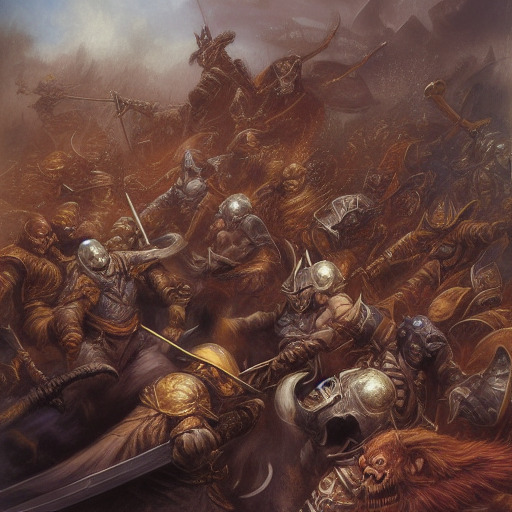
\includegraphics[width=\columnwidth]{introduction/simultaneous combat}
    In most TTRPGs, combat takes place in a series of turns.
    When your turn comes up, you take all of your actions, and then you wait through everyone else's turn until your turn comes again.
    This system has one foundational disadvantage: it is very, very slow.
    Rise uses a simultaneous combat system that dramatically increases the pace of combat.

    Imagine a typical 4-5 player game with 1-2 enemy groups using a traditional turn-based initiative system.
    In this scenario, you have to wait through about 5 turns before it comes back to your turn.
    This number can increase significantly in large-scale fights.
    Each of those 5 or so turns can meaningfully change the battlefield situation on its own by moving, weakening, or defeating various enemies and allies.
    The state of the battlefield at the end of last turn is often drastically different than the state of that battlefield at the start of your new turn.
    Player coordination can be challenging, since they must coordinate in the specific order assigned by the initiative system, and enemy turns can intervene to ruin coordinated plans.

    In theory, every player should accurately track the unfolding battlefield state through each of the intervening turns.
    That would mean everyone would know what to do when their turn comes up.
    In practice, many players find that difficult or impossible.
    Instead, at the start of each of their turns, they ask or try to figure out how the situation has changed.
    Not everyone asks this explicitly, but it must always be analyzed anew.

    Once a player understands the current battlefield state, they can finally decide their actions.
    This typically involves both movement and any number of sequential attacks, so there are many factors to consider.
    Everyone else must wait and do nothing while this happens.
    Once the active player has decided their actions, those actions must be fully rolled and resolved before combat can proceed.
    Even the next player in the initiative order may not be able to make accurate plans during this time, since the die rolls can change those plans.
    All of this combines to make even short combats take an hour or more, and six-person adventuring groups can feel dangerously bloated.

    Rise works differently.
    Combat in Rise is broken up into two phases: the movement phase and the action phase.
    During the movement phase, all creatures move simultaneously, and no attacks are possible.
    Characters can declare certain simple reactive movements like ``stay adjacent to this enemy'' to ensure that they end up in a reasonable position regardless of enemy actions.
    If the movements of characters conflict in impossible ways, initiative checks can temporarily force a linear order of resolution.
    Each player declares their own actions in an arbitrary order as soon as they decide them, so people are not forced to wait and do nothing while slower players contemplate their choices.
    Player coordination is easy, since all actions are happening together.

    During the action phase, players resolve their actions sequentially, but in an arbitrary order of the players' choice.
    This allows slower players to make their decisions when they are ready, while allowing faster players to resolve their actions first.
    Since movement during the action phase is rare, and enemies cannot unexpectedly move, players are typically able to decide their actions much more quickly and easily even when they have a large number of unique abilities to choose from.
    Once all players have resolved their actions, they learn what their enemies did.
    Those actions all resolve simultaneously, so enemy actions cannot interrupt player actions and vice versa.
    Attackers are always responsible for rolling instead of using ``saving throws'' or similar mechanics that force defenders to roll dice.
    All of this means that players can choose and resolve their actions simultaneously and efficiently, minimizing total time spent in combat while still allowing significant tactical complexity.

    The start of each phase still requires a general assessment from all acting players about the current state of the battlefield, which takes just as much time as the assessment in a classic initiative system.
    However, the time required for this tactical analysis only increases marginally as the number of players and enemies in the game increases.
    This allows Rise to handle large player counts or large enemy hordes without becoming glacially slow.
    Combat in Rise flows by quickly, making it much easier to balance time between combat and non-combat encounters within the same game session - or to run through multiple separate, individually challenging combats without sacrificing the pace and energy of the game.

  \subsection{Optional Complexity}
    Many games operate at a consistent level of complexity.
    Many rules-light games are always simple, and many rules-dense games are always complex.
    This is a perfectly reasonable design philosophy.
    Among other benefits, it makes it easy to know what to expect from the game, which helps give the game a well-defined niche.

    Rise is designed to allow players to choose their own level of complexity.
    This broadens its potential audience by allowing people with very different play styles or tolerances for complexity to enjoy the same game together.
    This goal is manifested in several key ways in Rise's design:
    \begin{itemize}
      \item Core gameplay is designed to be simple.
      \item Character creation is deeply interconnected.
      \item Complexity is not tied to narrative roles.
      \item Character power does not require complexity.
    \end{itemize}

    \subsubsection{Simple Core Gameplay}
      The core gameplay loop must be simple.
      You can contribute in combat by relying on one or two standard attacks that you use in all circumstances.
      In narrative situations, you can just roll the skills you have trained, and ignore other options.
      Engaging with the system more deeply than that is a choice, not a requirement.

    \subsubsection{Interconnected Character Creation}
      Character creation and build optimization is a better place to store complexity.
      Creating a Rise character involves a number of decisions, each of which can have nuanced ramifications on other aspects of the system.
      If you are just trying to build a character that matches a desired narrative, you can generally approach each decision in isolation.

      For example, you can decide that your character is intelligent and agile but not very strong or durable, because that is the concept you want.
      That decision has consequences, such as changing how many trained skills you have and what your defenses are.
      If you approach each decision sequentially, each one is relatively easy to make, and doesn't require deep system knowledge.
      On the other hand, trying to mathematically optimize a character requires thinking about many aspects of the system at once.
      This results in a system that is easy to learn but hard to master.

      Even for simple characters, the process of character creation is still one of the most complicated aspects of Rise.
      That is why Rise provides (or will provide, once that section is done) an extensive selection of premade characters for a wide variety of narrative archetypes.
      Each premade character includes advice for how to play that character and level them up.
      The premade characters make the system more accessible to people who don't want to to deal with the complexity of creating a character from scratch.

    \subsubsection{Complexity and Narrative}
      Complexity and simplicity should not be directly connected to a character's concept or narrative.`
      For example, it would be a bad idea to define a system where martial characters are simple and spellcasters are complicated.
      Both of those are rich and evocative narrative constructs.
      Many people who don't enjoy complexity will want to play spellcasters, and many people who enjoy complexity will want to play martial characters.
      Gameplay complexity must be more finely tuned and localized than those sweeping strokes.

      In Rise, gameplay complexity is generally generated by acquiring a large number of increasingly situational abilities.
      Every class has some archetypes that grant additional abilities known and some archetypes that grant additional passive abilities.
      If you like having a lot of unique abilities, you can have a high Intelligence to maximize your insight points, and focus on learning spells and maneuvers that attack your enemies or have situational effects.
      If you like minimizing complexity, you can instead choose archetypes or learn spells that simply grant you passive benefits, and focus on one or two standard attacks that you specialize in.
      Some feats give you new abilities and new circumstances to pay attention to that make you more effective, while others simply increase your passive statistics and defenses.

      Rise specifically handles complexity for martial characters and spellcasters slightly differently.
      Martial characters in Rise typically have fairly simple individual abilities.
      However, they can use those abilities with a variety of meaningfully different weapons.
      A martial character with four unique attacks and three different weapons has twelve different options in combat.
      In addition, martial characters can typically make better use of universal abilities, such as shoving and grappling.

      Spellcasters have more complex and varied individual abilities.
      They also tend to have more abilities that have significant narrative effects.
      However, their abilities are more isolated.
      There is no spellcaster equivalent of martial weapons that would multiply their number of distinct abilities in combat.
      The result of this design is that both martial characters and spellcasters can be very simple or very complicated.
      However, they approach complexity in different ways, ensuring that they feel narratively distinct.

    \subsubsection{Complexity and Power}
      All of this customization of complexity would be mostly pointless if complexity was strongly correlated with character power.
      If exceptionally complicated or hyper-specialized characters were obviously and consistently more effective than other characters, it would push everyone to use those characters.
      Rise structures the tradeoffs between gaining raw power and gaining additional options balanced enough that neither is always superior.

      There will always be some benefit from build optimization and system mastery.
      Players who are deeply familiar with Rise will be able to build characters with more relevant strengths and fewer relevant weaknesses.
      However, the gap between optimized characters and ``normal'' characters is limited.
      There will always be specific contexts where one character's mechanics are superior to another's.
      For example, a specialized defensive melee character may excel in a duel in a confined space.
      However, it may be irrelevant against cavalry archers on an open field.
      Characters in Rise cannot drastically change their capabilities each day, so they will always have moments to shine and moments of weakness.

  \subsection{Unbounded Scaling}
    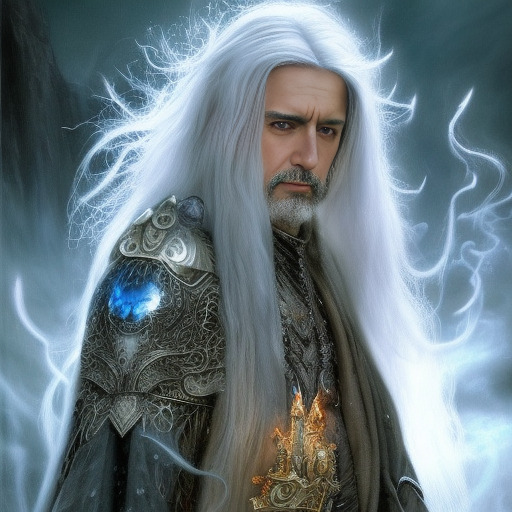
\includegraphics[width=\columnwidth]{introduction/unbounded scaling}
    Some systems uses bounded bonuses for accuracy or other game statistics.
    Bounded scaling means that every character of the same power level - or in some systems, of any power level - has a similar chance of success with any given skill check or attack roll.
    This can frequently cause narratively inappropriate and even comical events, and Rise explicitly rejects this philosophy.

    Imagine a typical party of four players, with one character being exceptionally skilled at a particular task.
    Perhaps the rogue is exceptionally skilled at lying, or a barbarian is exceptionally skilled at climbing.
    If ``exceptionally skilled'' only means that they have a \plus5 bonus on a d20 compared to \plus0 from the rest of the party, the exceptionally skilled character will only get the best result in the party half the time.
    The other half of the time, some other character with no relevant skills will meet or exceed the skilled character's result - sometimes by a dramatic margin.
    When failure compared to rank amateurs happens this often, it becomes hard to take seriously the idea that any character can be exceptionally skilled at anything.

    Rise characters can have dramatic statistical differences between each other, even at low levels.
    It uses a d10 as the fundamental die, which makes every bonus more significant.
    In addition, a 1st-level character can easily reach a \plus6 bonus with a skill check that is particularly relevant to their character.
    This means that a skilled character can beat a party of rank amateurs 80\% of the time, and at higher levels their success becomes completely guaranteed.
    Likewise, the difference in Mental defense between a powerful sorcerer and a cowardly rogue can allow mind-affecting attacks to almost always hit a rogue while almost never hitting the sorcerer.
    These statistical differences do not always grow with level, but they remain significant at every level.

    One advantage of systems with bounded scaling is that it is easier to guarantee that every character is relevant in any situation.
    Even if your character has no useful abilities of any kind, you might sometimes succeed on important actions through sheer luck.
    However, this design philosophy often breaks the symmetry between magical and non-magical characters.
    Magical characters can often use extremely specific and powerful abilities that are impossible for nonmagical characters to duplicate.
    If magical characters also have similar odds of success with all generic mechanics of the game, they will almost certainly have far more influence over the narrative of the game than any nonmagical character can hope to match.

    The philosophy of Rise is that it's okay for some characters to be irrelevant in specific contexts.
    It's good to give people time in the spotlight where their character's abilities help solve the specific problem that the group is facing when no other character could.
    Rise encourages that, and makes it impossible for one character to be relevant in \textit{all} contexts.
    Each character has their own strengths and weaknesses, and if you try to be good at everything, you'll fall behind people who specialize in a particular area.
    This will naturally rotate the spotlight between different characters, allowing each player to feel relevant and important in turn.

    This dramatic scaling is also used to govern the power of characters over time, in addition to the power of characters relative to each other.
    Rise attempts to model a massive power range for player characters.
    They are expected to start their journeys at level 1 as little more than commoners, and by level 21 they are effectively demigods who can alter the fate of entire worlds.
    This is a critical part of the narrative fabric of Rise, and it is reflected in the statistics and abilities of characters.
    If a level 1 kobold posed even a tiny threat to a level 21 character, the mechanics of the game would sabotage the purported narrative of power and growth.
    In Rise, overall character power doubles approximately every two to three levels.
    The system takes some care to avoid bloating numbers to unwieldy levels on this journey, and the use of the d10 as the standard die helps immensely.

  \subsection{Bounded Action Economy}
    It is dangerous to to give characters too many actions each turn.
    Each additional action a character can take increases how difficult it is for a player to decide what to do on their turn.
    In addition, each additional action increases the complexity of the change between the start of the turn and the end of the turn.
    This is especially risky with Rise's simultaneous initiative system, which combines the actions taken by all characters into a single resolution process.

    Rise places significant limitations on how many relevant actions each character can take on their turn.
    Generally, characters can only move during the movement phase and then take one significant action each turn.
    Some characters can use a minor action to accomplish something useful.
    However, that essentially marks the end of action economy scaling, even up to the maximum level.

    Detrimental effects that could deny actions are also heavily limited.
    Total action denial effects are only usable by high level characters, and even then they only work against weak enemies or enemies that have already been significantly damaged.
    Taking actions is fun, and sitting quietly while everyone else does things can be very frustrating.
    Similarly, completely removing an enemy's ability to act can easily remove the tension from a fight before it's actually over.
